\documentclass[10pt]{article}

\usepackage[margin=1in]{geometry} 
\usepackage{amsmath,amsthm,amssymb,bbm,subfig,graphicx,float,physics,listings,fontspec,color}
\newfontfamily\Consolas{Consolas}
\definecolor{grey}{rgb}{0.9,0.9,0.9}
\lstset{basicstyle=\ttfamily, breaklines=true, numbers=left, numberstyle=\ttfamily, backgroundcolor=\color{grey}\ttfamily, keywordstyle=\color{blue}\ttfamily, stringstyle=\color{red}\ttfamily, commentstyle=\color{green}\ttfamily}
\DeclareMathOperator*{\argmin}{arg\,min}
\DeclareMathOperator*{\argmax}{arg\,max}
\DeclareMathOperator*{\vari}{var}

\begin{document}


% --------------------------------------------------------------
%                         Start here
% --------------------------------------------------------------
 
%\renewcommand{\qedsymbol}{\filledbox}
 
\title{\textbf{Report on Project 1}}%replace X with the appropriate number
\author{Zhunxuan Wang, 13300180086\\ %replace with your name
School of Mathematical Sciences} %if necessary, replace with your course title

\maketitle
\section{Linear Regression and Nonlinear Bases}
\subsection{Adding a Bias Variable}
Based on the model in the original function \texttt{leastSquares}
$$\hat{\mathbf{y}} = \mathbf{X}\hat{\mathbf{w}}\text{,}$$
and the minimization of the loss
$$\min_{\mathbf{w}}\norm{\mathbf{y} - \mathbf{X}\mathbf{w}}_2^2$$
of which the explicit solution \cite{shumway2010time} is
\begin{equation}
\hat{\mathbf{w}} = \left(\mathbf{X}^\intercal\mathbf{X}\right)^{-1}\mathbf{X}^\intercal\mathbf{y}\text{.}
\label{equ_1}
\end{equation}
I inserted a vector with all ones in the first column of $\mathbf{X}$, then the first dimension of $\hat{\mathbf{w}}$ would be fitted as the bias term
$$\hat{\mathbf{y}} = \begin{pmatrix}
\mathbf{1} & \mathbf{X}
\end{pmatrix}\begin{pmatrix}
\beta \\
\hat{\mathbf{w}}
\end{pmatrix}$$
where $\beta$ is the bias term. The exact solution is in the same form as equation \ref{equ_1}. And the updated plot is shown as follows
\begin{figure}[H]
\centering
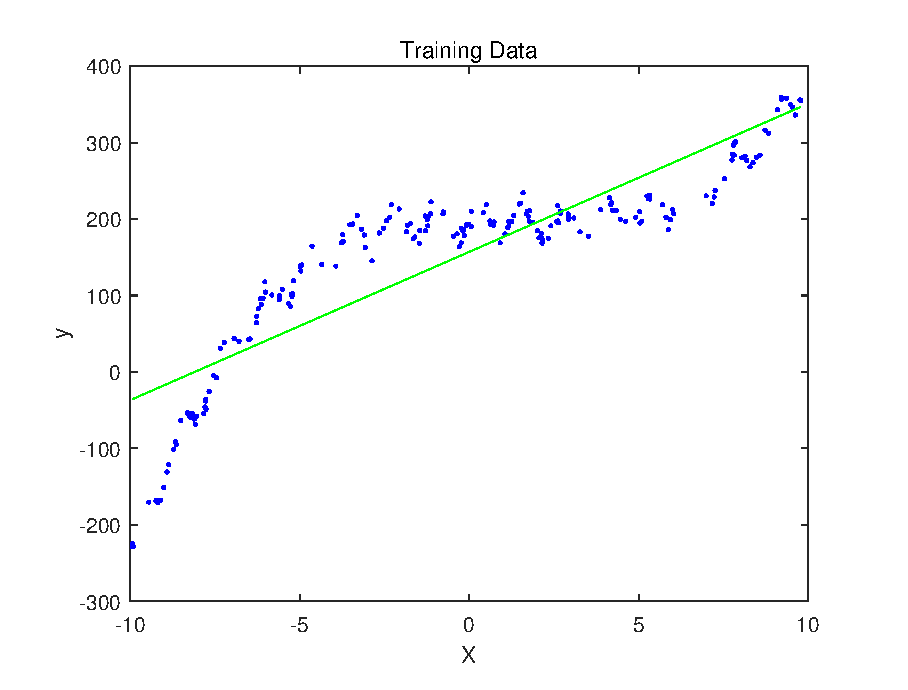
\includegraphics[scale=.65]{plot1_1.eps}
\caption{The Fitting (with Bias) Plot}
\label{plot1_1}
\end{figure}
The training error of the fitting above is $3551.35$, and the test error is $3393.87$.\par
The code of function \texttt{leastSquaresBias} is shown as follows
\begin{lstlisting}[language=MATLAB]
function [model] = leastSquaresBias(X, y)

% append a vector to the first column
X_app = [ones(size(X, 1), 1) X];

% calculate the estimated weight values
w_bias = (X_app' * X_app) \ X_app' * y;

% weight values with bias
model.w_bias = w_bias;
model.predict = @predict;

end

function [y_hat] = predict(model, X)

% append a vector to the first column
X_app = [ones(size(X, 1), 1) X];

% make prediction
y_hat = X_app * model.w_bias;

end
\end{lstlisting}
\subsection{Polynomial Basis}
Linear fitting does not work well when the complexity of the data is considerably high. Thus we consider fitting a polynomial model. E.g., when the degree of the polynomial is $3$, this model will be
$$\hat{\mathbf{y}} = \mathbf{X}_{\text{poly}}\hat{\mathbf{w}}$$
where
$$\mathbf{X}_{\text{poly}} = \begin{bmatrix}
1 & x_1 & x_1^2 & x_1^3 \\
1 & x_2 & x_2^2 & x_2^3 \\
\vdots & \vdots & \vdots & \vdots \\
1 & x_n & x_n^2 & x_n^3 \\
\end{bmatrix}\text{.}$$
The explicit solution would still be
$$\hat{\mathbf{w}} = \left(\mathbf{X}_{\text{poly}}^\intercal\mathbf{X}_{\text{poly}}\right)^{-1}\mathbf{X}_{\text{poly}}^\intercal\mathbf{y}\text{,}$$
and the fitted curve is a cubic curve. It will be similar cases if the polynomial degree is greater.\par
The training error and the test error against \texttt{deg} are shown as follows
\begin{center}
\resizebox{\textwidth}{!}{
\begin{tabular}{|c|c|c|c|c|c|c|c|c|c|c|c|}
\hline
deg & $0$ & $1$ & $2$ & $3$ & $4$ & $5$ & $6$ & $7$ & $8$ & $9$ & $10$ \\
\hline
training & $15480.52$ & $3551.35$ & $2167.99$ & $252.05$ & $251.46$ & $251.14$ & $248.58$ & $247.01$ & $241.31$ & $235.76$ & $235.07$ \\
\hline
test & $14390.76$ & $3393.87$ & $2480.73$ & $242.80$ & $242.13$ & $239.54$ & $246.01$ & $242.89$ & $245.97$ & $259.30$ & $256.30$ \\
\hline
\end{tabular}
}
\end{center}
And the smoothed log-error plot of the table above is shown as follows
\begin{figure}[H]
\centering
\includegraphics[scale=.65]{plot1_2.eps}
\caption{The Log-Error (against deg) Plot (smoothed)}
\label{plot1_1}
\end{figure}
As we observe from the table and the plot above, the errors showed a steep decreasing situation when \texttt{deg} was not greater than $3$, then showed an unconspicuous down trend for training error, and down-up trend for test error (may be a trend of overfitting). The optimal \texttt{deg} for test error is $5$, when the optimal test error is $239.54$. The code is shown as follows
\begin{lstlisting}[language=MATLAB]
function [model] = leastSquaresBasis(X, y, deg)

% generate the polynomial-form matrix
X_app = zeros(size(X, 1), deg + 1);
for i = 0 : deg
  X_app(:, i + 1) = X .^ i;
end

% calculate the estimated weight values
w_bias = (X_app' * X_app) \ X_app' * y;

% weight values with bias
model.w_bias = w_bias;
model.deg = deg;
model.predict = @predict;

end

function [y_hat] = predict(model, X)

% generate the polynomial-form matrix
X_app = zeros(size(X, 1), model.deg + 1);
for i = 0 : model.deg
  X_app(:, i + 1) = X .^ i;
end

% make prediction
y_hat = X_app * model.w_bias;

end
\end{lstlisting}
\clearpage

\section{Ridge Regression}
For the ridge regression model, the hypothesis function is the same as linear regression
$$\hat{\mathbf{y}} = \mathbf{X}\hat{\mathbf{w}}\text{,}$$\par
Taking the sum of the loss of LR and an $L^2$-regularization term as the loss function
$$J\left(\mathbf{X},\mathbf{y};\, \mathbf{w}\right) = \norm{\mathbf{y} - \mathbf{X}\mathbf{w}}_2^2 + \delta^2\norm{\mathbf{w}}_2^2\text{,}$$
hence
$$\hat{\mathbf{w}} = \argmin_{\mathbf{w}}J\left(\mathbf{X},\mathbf{y};\, \mathbf{w}\right)\text{.}$$\par
We use matrix-form linear least squares method from \cite{shumway2010time}
$$\hat{\mathbf{w}} = \left(\mathbf{X}^\intercal\mathbf{X} + \delta^2\mathbf{E}\right)^{-1}\mathbf{X}^\intercal\mathbf{y}\text{.}$$
\subsection{Preprocessing}
We take the prostate cancer dataset, constructing a model to predict the $9$-th variable a linear combination of the other $8$. Before the model training, we shuffle the table, split the dataset to training and testing set, and take the standard score for each attribute of $\mathbf{X}$, and demean $\mathbf{y}$
$$\left(X_{\text{std}}\right)_{i,j} = \frac{X_{i,j} - \bar{X}_j}{\sigma_j},\, \left(y_{\text{std}}\right)_i = y_i - \bar{y}\text{,}$$
where $\bar{X}_j$ and $\sigma_j$ are the mean and the standard deviation of the $j$-th attribute in $\mathbf{X}$ respectively, $\bar{y}$ is the mean of $\mathbf{y}$.
\subsection{Training and Testing}
By tuning the regularization parameter $\delta^2$ from $10^{-2}$ to $10^4$ and training, we have the regularization path of each parameter and the training and test error against $\log_{10}\delta^2$ for ridge regression
\begin{figure}[H]
\centering
\begin{minipage}[b]{0.45\textwidth}
\centering
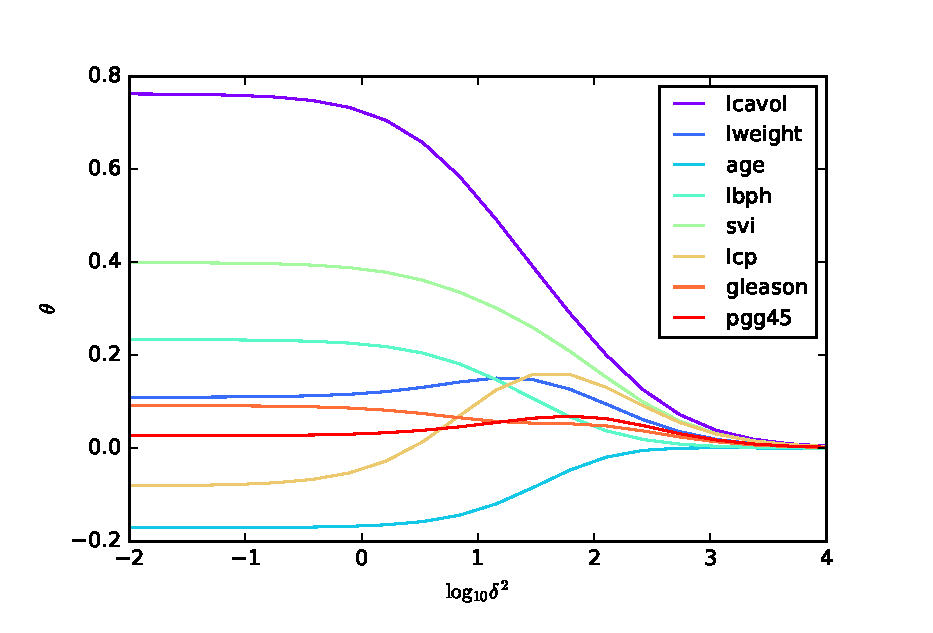
\includegraphics[scale=.5]{plot2_1.eps}
\caption{Regularization Path of Each Parameter}
\label{plot2_1}
\end{minipage}
\
\begin{minipage}[b]{0.45\textwidth}
\centering
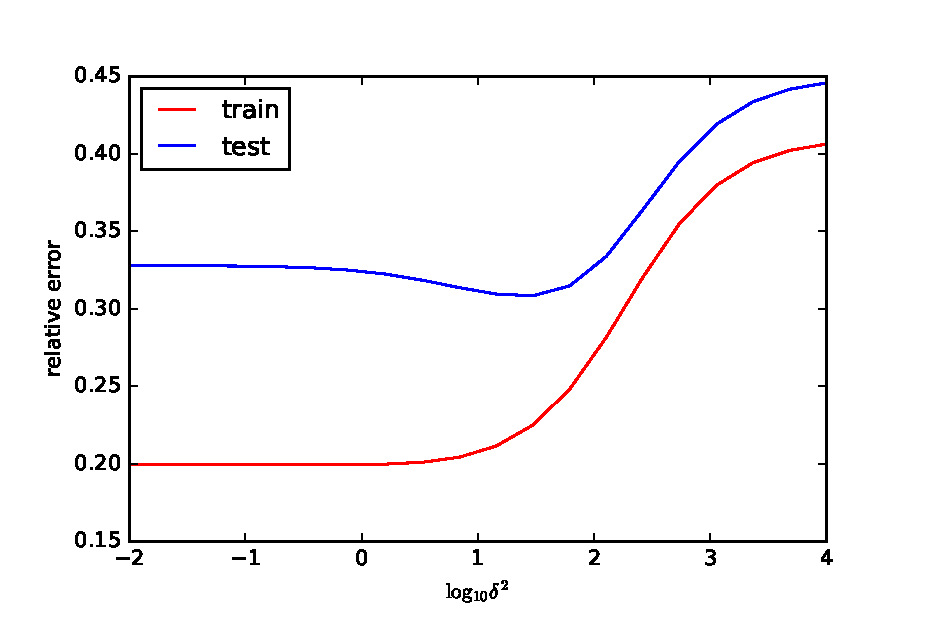
\includegraphics[scale=.5]{plot2_2.eps}
\caption{The Error Plot against $\log_{10}\delta^2$}
\label{plot2_2}
\end{minipage}
\end{figure}
As we observe from the plots above, the regularization path of each parameter shows a steady state when $\log_{10}\delta^2 < 0$ (so as the errors), and then a convergence trend to zero. The errors show a increasing trend when $\log_{10}\delta^2 > 1.5$, and the test error is permanently greater than the training error in this experiment.
\subsection{Cross Validation}
Applying the $k$-fold cross validation \cite{kohavi1995study} (set $k = 10$) to choose the parameter
\begin{itemize}
\item Fix the regularization parameter $\delta^2$.
\item Randomly divide the dataset into $k$ sets with similar size.
\item Take each single set as the test set, and take the rest folds as the training set, iteratively.
\item After $k$ times of training, calculate the mean of test errors in the $k$ times.
\item Try other regularization parameter $\delta^2$, and repeat the steps obtaining the mean of test errors.
\item Criterion to choose $\delta^2$: Choose the parameter with the minimum mean of test errors.
\end{itemize}
Tuning the regularization parameter $\delta^2$ from $10^{-2}$ to $10^4$ and training, we have the plot of means of test errors against $\log_{10}\delta^2$
\begin{figure}[H]
\centering
\includegraphics[scale=.65]{plot2_3.eps}
\caption{Mean relative error against $\log_{10}\delta^2$}
\label{plot2_3}
\end{figure}
On this dataset, based on the the criterion, optimal $\delta^2 = 10^{1.158}$, when the mean relative error is $0.276422$.
\clearpage
\footnotesize
\bibliographystyle{plain}
\bibliography{ref}

\end{document}